%% 
%% Copyright 2007-2020 Elsevier Ltd
%% 
%% This file is part of the 'Elsarticle Bundle'.
%% ---------------------------------------------
%% 
%% It may be distributed under the conditions of the LaTeX Project Public
%% License, either version 1.2 of this license or (at your option) any
%% later version.  The latest version of this license is in
%%    http://www.latex-project.org/lppl.txt
%% and version 1.2 or later is part of all distributions of LaTeX
%% version 1999/12/01 or later.
%% 
%% The list of all files belonging to the 'Elsarticle Bundle' is
%% given in the file `manifest.txt'.
%% 

%% Template article for Elsevier's document class `elsarticle'
%% with numbered style bibliographic references
%% SP 2008/03/01
%%
%% 
%%
%% $Id: elsarticle-template-num.tex 190 2020-11-23 11:12:32Z rishi $
%%
%%
\documentclass[preprint,12pt]{elsarticle}

%% Use the option review to obtain double line spacing
%% \documentclass[authoryear,preprint,review,12pt]{elsarticle}

%% Use the options 1p,twocolumn; 3p; 3p,twocolumn; 5p; or 5p,twocolumn
%% for a journal layout:
%% \documentclass[final,1p,times]{elsarticle}
%% \documentclass[final,1p,times,twocolumn]{elsarticle}
%% \documentclass[final,3p,times]{elsarticle}
%% \documentclass[final,3p,times,twocolumn]{elsarticle}
%% \documentclass[final,5p,times]{elsarticle}
%% \documentclass[final,5p,times,twocolumn]{elsarticle}

%% For including figures, graphicx.sty has been loaded in
%% elsarticle.cls. If you prefer to use the old commands
%% please give \usepackage{epsfig}

%% The amssymb package provides various useful mathematical symbols
\usepackage{amssymb,amsthm,amsmath}
%% The amsthm package provides extended theorem environments
%% \usepackage{amsthm}
% The float package adjusts figures' positioning
\usepackage{float}
% The mchem package adds support for displaying chemistry notations
\usepackage[version=4]{mhchem}
\usepackage{cleveref}

% \usepackage[linesnumbered, algochapter, ruled, longend]{algorithm2e}
% \usepackage{cleveref}
% \usepackage{tabularx}

%% The lineno packages adds line numbers. Start line numbering with
%% \begin{linenumbers}, end it with \end{linenumbers}. Or switch it on
%% for the whole article with \linenumbers.
%% \usepackage{lineno}

\journal{Tomography of Materials and Structures}

\begin{document}

\begin{frontmatter}

%% Title, authors and addresses

%% use the tnoteref command within \title for footnotes;
%% use the tnotetext command for theassociated footnote;
%% use the fnref command within \author or \address for footnotes;
%% use the fntext command for theassociated footnote;
%% use the corref command within \author for corresponding author footnotes;
%% use the cortext command for theassociated footnote;
%% use the ead command for the email address,
%% and the form \ead[url] for the home page:
%% \title{Title\tnoteref{label1}}
%% \tnotetext[label1]{}
%% \author{Name\corref{cor1}\fnref{label2}}
%% \ead{email address}
%% \ead[url]{home page}
%% \fntext[label2]{}
%% \cortext[cor1]{}
%% \affiliation{organization={},
%%             addressline={},
%%             city={},
%%             postcode={},
%%             state={},
%%             country={}}
%% \fntext[label3]{}

\title{Particle Pack Generation: Synthesise Tomograms with Physics-Based Simulation}

%% use optional labels to link authors explicitly to addresses:
%% \author[label1,label2]{}
%% \affiliation[label1]{organization={},
%%             addressline={},
%%             city={},
%%             postcode={},
%%             state={},
%%             country={}}
%%
%% \affiliation[label2]{organization={},
%%             addressline={},
%%             city={},
%%             postcode={},
%%             state={},
%%             country={}}

\author[inst1]{Bogong Wang}
\author[inst2]{Andrew Kingston}
\author[inst2]{Philipp L\"{o}sel}
\author[inst1]{Warren Creemers}

\affiliation[inst1]{organization={School of Computing},%Department and Organization
            addressline={The Australian National University}, 
            city={Canberra},
            postcode={2617}, 
            state={ACT},
            country={Australia}}

\affiliation[inst2]{organization={Research School of Physics},%Department and Organization
            addressline={The Australian National University}, 
            city={Canberra},
            postcode={2617}, 
            state={ACT},
            country={Australia}}


\begin{abstract}
%% Text of abstract
In the field of geology, 3D imaging of geological particle samples by computed tomography (CT) offers the means for non-destructive analysis. 
However, obtaining such tomograms with the corresponding segmentation labels remains a significant challenge. 
% Current methods are constrained by the need for extensive manual inspection and correction, as the initial segmentation is often inaccurate.
This study introduces a novel physics-based simulation workflow that generates synthetic tomograms with segmentation ground truths. 
% By simulating the physical particle packing process, we produce enriched datasets that improve segmentation accuracy. 
The synthetic dataset enriches the existing data resources in the field, offering potential benefits for data-intensive applications, such as machine learning.
\end{abstract}

%%Graphical abstract
\begin{graphicalabstract}
\begin{figure}[H]
    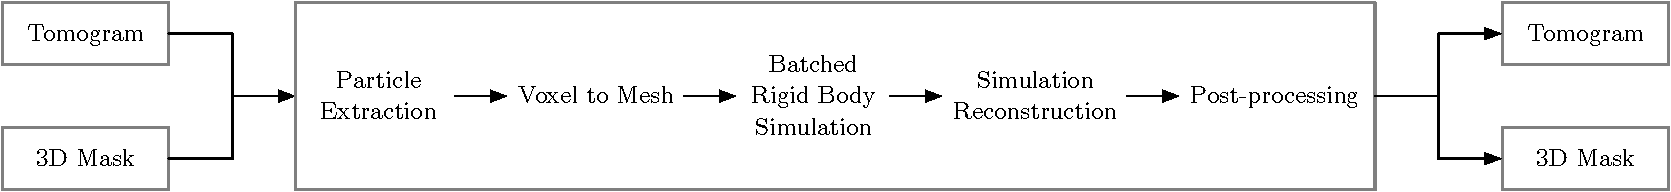
\includegraphics[width=\textwidth]{./figures/pdf/synthesis-workflow.pdf}
\end{figure}
\end{graphicalabstract}

%%Research highlights
\begin{highlights}
    % \item We presented the Particle Pack Dataset, comprising micro-CT scans of crushed quartz. The dataset presents segmentation challenges due to the variability in particle shape and size..
    \item We introduced a novel workflow that generates synthetic tomograms with segmentation ground truths. This method enriches existing tomographic datasets, offering substantial benefits for machine learning and data-intensive applications such as geology and materials science.
    % \item We introduced a method for generating synthetic particle packs from the existing dataset, thereby facilitating further research in the field of machine learning.
\end{highlights}

\begin{keyword}
%% keywords here, in the form: keyword \sep keyword
Computed Tomography \sep ???
%% PACS codes here, in the form: \PACS code \sep code
% \PACS 0000 \sep 1111
%% MSC codes here, in the form: \MSC code \sep code
%% or \MSC[2008] code \sep code (2000 is the default)
% \MSC 0000 \sep 1111
\end{keyword}

\end{frontmatter}

%% \linenumbers

%% main text
\section{Introduction} \label{sec:introduction}
In geology, the use of computed tomography (CT) to scan geological particle samples has become increasingly common \cite{VANGEET200025, cnudde20123d, warlo2021multi}.
CT scanning offers the significant advantage of providing 3D non-destructive inspection of large batches of particle samples, often referred to as particle packs.
However, to perform comprehensive analyses of these particle packs, it is essential to accurately segment individual particles. 
This segmentation is crucial for examining specific attributes such as composition and physical properties.

As the utilisation of machine learning expands, there is an increasing demand for comprehensive datasets.
A significant challenge in this context is acquiring CT volumes or tomograms and the precise segmentation ground truth.
Obtaining tomograms involves complex processes, specialised users and sophisticated equipment, which can be costly to run and resource-intensive. 
Additionally, achieving accurate segmentation with current methods, such as the watershed algorithm, often requires laborious manual corrections.

In this work, we present a novel approach that utilises a physics-based simulation engine to synthesise tomograms with corresponding segmentation ground truths. 
This method generates synthetic particle pack data, enriching the available particle pack datasets in various fields.


%%%%%%%%%%%%%%%%%%%%%%%%%%%%%%%%%%%%%%%%%%%%%%%%%%%%%%%%%%%%%%%%%%%%%%%%%%%%%%%%
%%%%%%%%%%%%%%%%%%%%%%%%%%%%%%%%%%%%%%%%%%%%%%%%%%%%%%%%%%%%%%%%%%%%%%%%%%%%%%%%
%%%%%%%%%%%%%%%%%%%%%%%%%%%%%%%%%%%%%%%%%%%%%%%%%%%%%%%%%%%%%%%%%%%%%%%%%%%%%%%%
\section{Background}
Synthetic data generation is a promising solution to address the inherent difficulties in collecting realistic and unbiased particle pack datasets.
\par
Simulation-based methods are commonly used in synthetic data generation \citep{demelo2022nextgeneration}.
These methods employ computational models such as physics simulators or scene rendering engines to generate synthetic data that mimic real-world scenarios or phenomena for custom domains. 
The core idea is to create a virtual environment that replicates physical dynamics or real-world scenes accurately.
% commonly used simulation based tools
Common tools include physical simulation engines such as Bullet Engine \citep{coumans2021pybullet} and PhysX \citep{nvidia2024nvidia} that are used for their physics modeling capabilities such as rigid body simulation or particle dynamics simulation. 
Additionally, game engines like Unity \citep{unity2024unity} and Unreal Engine \citep{unreal2024epic} are also frequently utilised, offering rendering capabilities to simulate realistic scenes or environments.
% successfully deployed tasks
% \par
% These simulation-based approaches have shown considerable success in various applications. 
% For instance, they are critical in generating annotated images for training object detection models in autonomous driving \citep{richter2016playing, abualhaija2018augmented}.
\par
% pros and cons
One of the main advantages of simulation-based methods is their high level of controllability \citep{muller2018sim4cv}.
By allowing precise control over both the data generation process and the characteristics of the generated data, researchers and developers can ensure that the output closely adheres to specific criteria or regulatory requirements. 
This transparency is crucial in understanding exactly how the data was produced, which is particularly beneficial in regulated industries where proving data integrity and compliance is essential. 
Additionally, simulation-based methods are advantageous because they do not necessarily require large initial datasets. 
Unlike methods that rely heavily on existing large volumes of data, simulations can generate valuable synthetic data from theoretical models or smaller existing datasets. 
This capability is particularly useful in scenarios where real data is scarce or difficult to obtain.
\par
However, simulation-based methods have disadvantages.
The complexity of creating accurate simulations represents a significant challenge \citep{demelo2022nextgeneration}; it is often a complex and time-consuming process that demands a thorough understanding of the underlying physical or logical processes that the data aims to represent. 
Such complexity can limit the speed and scalability of data generation initiatives.
Moreover, the novelty of data produced by simulation-based methods is inherently limited by the assumptions and rules embedded within the simulation data and models. 
As a result, these methods might restrict the ability to uncover unexpected patterns or anomalies within the data, potentially leading to insights that are biased towards pre-conceived notions encoded in the simulation framework. 
This limitation is particularly relevant in fields where discovering novel insights and understanding previously unrecognised phenomena are the primary objectives.


%%%%%%%%%%%%%%%%%%%%%%%%%%%%%%%%%%%%%%%%%%%%%%%%%%%%%%%%%%%%%%%%%%%%%%%%%%%%%%%%
%%%%%%%%%%%%%%%%%%%%%%%%%%%%%%%%%%%%%%%%%%%%%%%%%%%%%%%%%%%%%%%%%%%%%%%%%%%%%%%%
%%%%%%%%%%%%%%%%%%%%%%%%%%%%%%%%%%%%%%%%%%%%%%%%%%%%%%%%%%%%%%%%%%%%%%%%%%%%%%%%
\section{Method}\label{sec:method}
\begin{figure}
    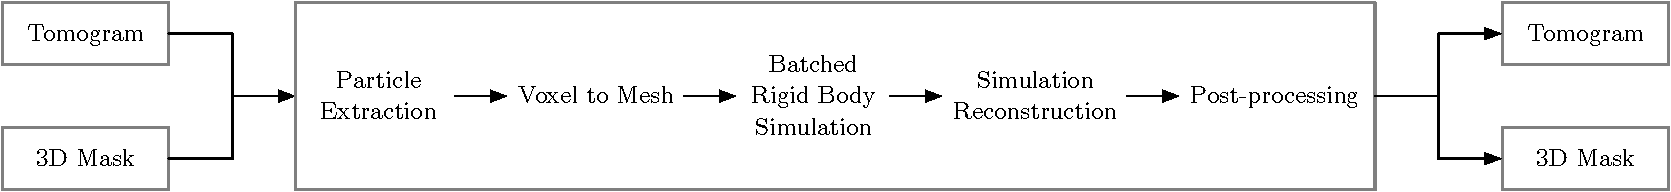
\includegraphics[width=\textwidth]{figures/pdf/synthesis-workflow.pdf}
    \caption{Particle Pack Synthesis Workflow}
    \label{fig:workflow}
\end{figure}
To enrich existing particle pack datasets, we propose a workflow for generating synthetic particle packs, as illustrated in \cref{fig:workflow}.
This workflow aims to replicate the physical particle packing process, which involves sifting particles based on their size and then pouring them into a cylinder for a CT scan.
\par
The process commences with the acquisition of a real particle pack volume (from a CT scan) and the corresponding labelled volume.
A labelled volume, also known as a ``mask'', assigns each particle in the particle pack a unique label.
To reduce the computational load in the simulation process, these extracted particle volumes are converted into meshes. 
A physics simulator then performs rigid body simulations on these meshes. 
This determines the rotations and positions of particles within the simulated tomogram.
Following this, the original particle volumes, masks and the simulation outcomes are used to reconstruct a synthetic tomogram and its 3D mask. 
The workflow concludes with a post-processing step, where modifications such as adding noise are applied to the reconstructed tomograms and masks to ensure that the output is realistic.
\par
In the following subsections, we will detail each subprocess including particle extraction, voxel to mesh conversion, batched rigid body simulation, simulation reconstruction and postprocessing.
%===============================================================================
\subsection{Particle Extraction} \label{sec:method:subsec:particle_extraction}
Particle extraction is the process of extracting a volume encompassing each particle from the tomogram and its mask.
The input of such a process is a tomogram-label pair, the output is a list of extracted particle volumes and their label volumes. 

As shown in \cref{fig:extract_particles}, the particle extraction process begins by identifying the bounding box of the particle from its mask. 
The mask and tomogram are then cropped using the bounding box to coarsely isolate from other particles.
Next, the binary mask of the target particle is created by eliminating the masks of surrounding particles.
This binary mask is subsequently applied to the cropped tomogram, producing a clean tomogram of the selected particle.

\begin{figure}
    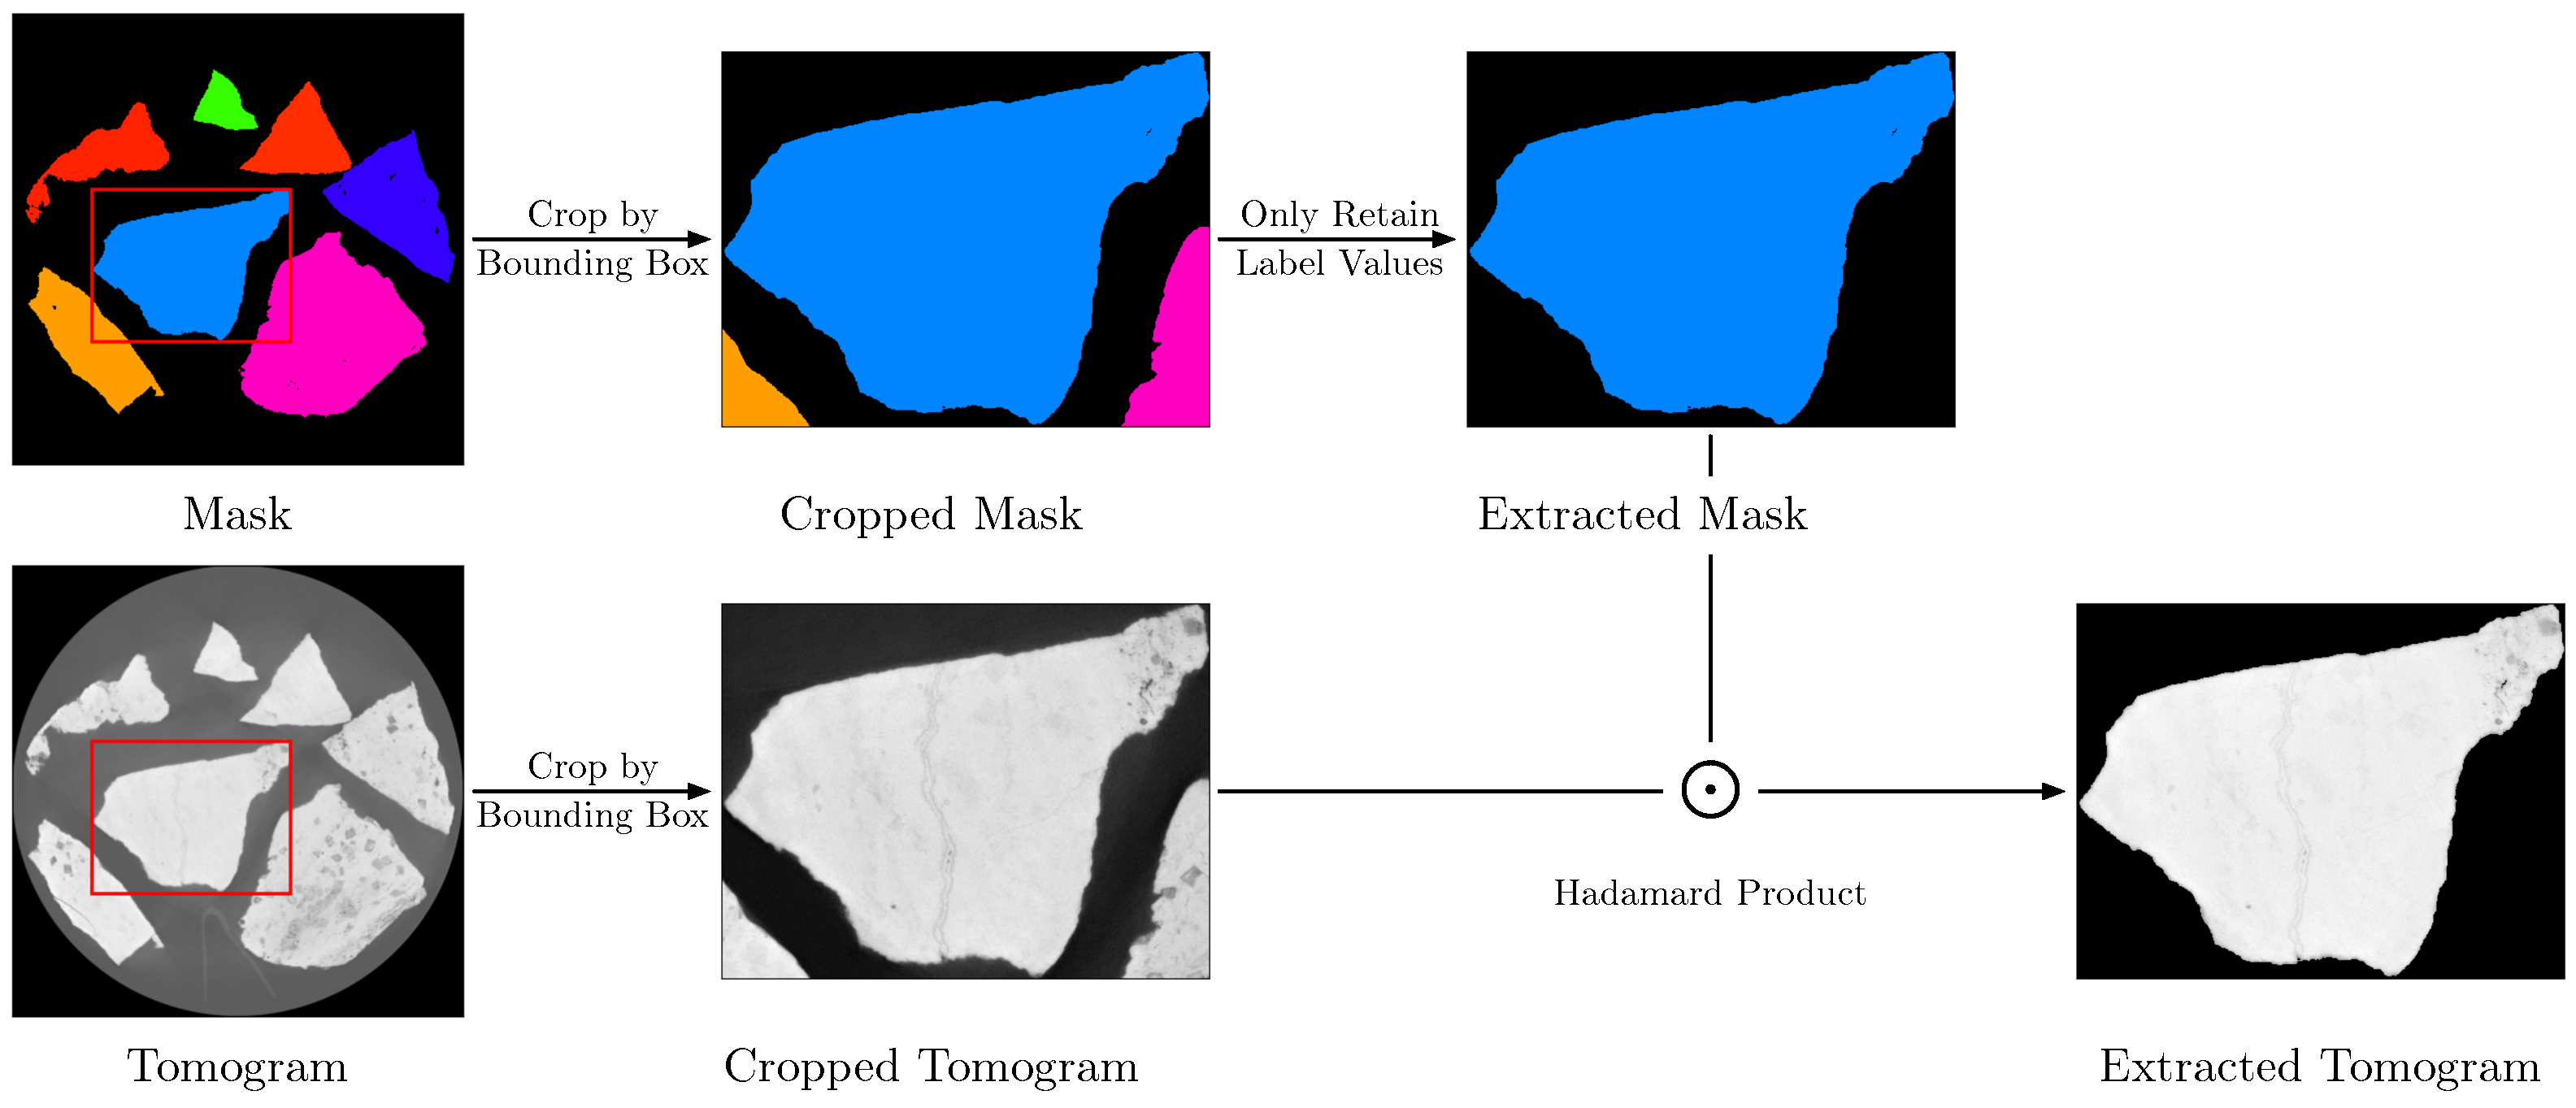
\includegraphics[width=\textwidth]{figures/pdf/particle-extraction.pdf}
    \caption{2D Illustration of Particle Extraction Process} \label{fig:extract_particles}
\end{figure}

% \par
% To efficiently extract the particles, it is advantageous to focus exclusively on the memory block that contains the particle targeted for extraction. 
% Therefore, identifying each particle's bounding box is crucial. 
% Consequently, we introduce a parallel, single-pass algorithm (\cref{alg:syn:find_bounding_boxes}) designed for efficient bounding box calculation for every particle.
% % \begin{algorithm}
% %     \SetKwFor{ParallelFor}{parallel for}{do}{end parallel for}
% %     \caption{Find Bounding Boxes(\it{Mask}, \it{n}, \it{xDim}, \it{yDim}, \it{zDim})}\label{alg:syn:find_bounding_boxes}
% %     \DontPrintSemicolon
% %     \KwIn{The mask (\it{Mask}) of a tomogram, the number of particles \it{n} and the $x, y$ and $z$ dimension (\it{xDim}, \it{yDim} and \it{zDim}) of the \it{Mask}}
% %     \KwOut{Bounding box for all particles in the mask.}
% %     Let $\it{BoundingBoxes}[1\dots n][1\dots 6]$ be new array \;
% %     $\it{BoundingBoxes}[\dots][1, 3, 5] = \infty$ \;
% %     $\it{BoundingBoxes}[\dots][2, 4, 6] = -\infty$ \;
% %     \ParallelFor {$1 \le x \le xDim$} {
% %         \For {$1 \le y \le yDim$} {
% %             \For {$1 \le z \le zDim$} {
% %                 label = \it{Mask}[\it{x}][\it{y}][\it{z}] \;
% %                 $\it{BoundingBoxes}[label][1] = \tt{Min}(\it{BoundingBoxes}[\it{label}][1], x)$ \;
% %                 $\it{BoundingBoxes}[label][2] = \tt{Max}(\it{BoundingBoxes}[\it{label}][2], x)$ \;
% %                 $\it{BoundingBoxes}[label][3] = \tt{Min}(\it{BoundingBoxes}[\it{label}][3], y)$ \;
% %                 $\it{BoundingBoxes}[label][4] = \tt{Max}(\it{BoundingBoxes}[\it{label}][4], y)$ \;
% %                 $\it{BoundingBoxes}[label][5] = \tt{Min}(\it{BoundingBoxes}[\it{label}][5], z)$ \;
% %                 $\it{BoundingBoxes}[label][6] = \tt{Max}(\it{BoundingBoxes}[\it{label}][6], z)$
% %             }
% %         }
% %     }
% %     \Return{\it{BoundingBoxes}}
% % \end{algorithm}
% \par
% After inspecting the \cref{alg:syn:find_bounding_boxes}, it is evident that the algorithm's complexity is \O{xyz}, where $x, y$ and $z$ represent the dimensions of the mask in three respective directions, because for each voxel in the input mask, the algorithm iterates only once.
% \par
% With the bounding boxes identified, we can efficiently extract particles and their corresponding masks. 
% As outlined in \cref{alg:syn:extract_particles}, the particle extraction process begins by detecting the label and bounding box of each particle from the input mask, then extracts and saves the particles in parallel. 
% The extraction involves cropping the tomogram and its mask using the pre-computed bounding boxes. 
% Given that the cropped areas may still contain multiple particles, we address this by retaining only the mask values that match the specific label, referred to as the ``extracted mask''. 
% Subsequently, an element-wise multiplication (Hadamard product, denoted as $\odot$) is performed between the extracted mask and the cropped tomogram to obtain the ``extracted tomogram'', as depicted in \cref{fig:syn:extract_particles}.

% % \begin{algorithm}
% %     \SetKwFor{ParallelFor}{parallel for}{do}{end parallel for}
% %     \caption{Extract Particles(\it{Tomogram}, \it{Mask})}\label{alg:syn:extract_particles}
% %     \DontPrintSemicolon
% %     \KwIn{The tomogram (\it{Tomogram}) contains particles, and its mask (\it{Mask}).}
% %     \KwOut{Separated particles in the tomogram with its mask in voxels.}
% %     $\it{labels} = \tt{UniqueValues}(\it{Mask})$ \;
% %     $\it{n} = \tt{Length}(\it{labels})$ \;
% %     $\it{xDim}, \it{yDim}, \it{zDim} = \tt{Dimension}(\it{Mask})$ \;
% %     $\it{boundingBoxes} = \tt{CalculateBoundingBoxes}(\it{Mask}, \it{n}, \it{xDim}, \it{yDim}, \it{zDim})$ \;
% %     \ParallelFor {$label \in labels$} {
% %         $\it{boundingBox} = \it{boundingBoxes}[label]$ \;
% %         $\it{croppedTomogram} = \tt{crop}(\it{Tomogram}, \it{boundingBox})$ \;
% %         $\it{croppedMask} = \tt{crop}(\it{Mask}, \it{boundingBox})$ \;
% %         $\it{extractedMask} =$ only retain values in $\it{croppedMask}$ equal to $label$ \;
% %         \tt{save}(\it{extractedMask}) \;
% %         % \tcp{$\odot$: Hadamard product}
% %         $\it{extractedTomogram} = \it{extractedMask} \odot \it{croppedTomogram}$ \; 
% %         \tt{save}(\it{extractedTomogram})
% %     }
% % \end{algorithm}

% In \cref{alg:syn:extract_particles}, \texttt{UniqueValues} function finds the indices of masks. 
% \texttt{Length} is to obtain the size of an array. 
% And function \texttt{Dimension} is used to find the $x, y$ and $z$ dimension of the input mask.

% Utilising pre-computed bounding boxes significantly simplifies the process of obtaining the \textit{croppedMask}, as we can exclusively focus on the memory block that corresponds to the mask, which reduces both the computational and memory complexity of processing \textit{croppedMask} from %\O{xyz} to \O{rst}. 
% Here, $x, y$ and $z$ represent the dimensions of the tomogram, while $r, s$ and $t$ denote the dimensions of the bounding box. 
% Consequently, the total complexity of the algorithm is given by \O{nrst}, where $n$ is the number of particles, and $r, s$ and $t$ correspond to the dimensions of the largest bounding box among the particles.
% % As extracting the number mask values requires iterating through the whole 
% % mask, results in a complexity of \O{xyz}.

%===============================================================================
\subsection{Volume to Mesh}
The conversion of extracted mask volumes into mesh structures is necessitated by the requirement for efficiency in rigid body simulations. 
The primary aim of these physics-based simulations is to accurately model the physics involved in the particle packing process. 
This include the collisions and interactions among particles. 
As a result, only the voxel surfaces and total mass are required in the simulation. 
\par
The conversion process for the entire tomogram can be efficiently parallelised for all particles. 
This is achieved by simultaneously extracting the volume of each particle and converting it to a mesh.
% The procedure is outlined in \cref{alg:syn:voxel_to_mesh}. 
The transformation of volumes into meshes is facilitated by employing the marching cubes algorithm \citep{lorensen1987marching}. 
Furthermore, to enhance simulation performance through a reduction in vertex points, mesh decimation techniques, as detailed by \citep{garland1997surface}, can be strategically utilised to decrease the vertex count while preserving the external geometry of the particle mesh. 
After obtaining the meshed particles, particle packing process can then be efficiently simulated. 

% \begin{algorithm}
%     \SetKwFor{ParallelFor}{parallel for}{do}{end parallel for}
%     \caption{Volume To Mesh(\it{ParticleMasks})}\label{alg:syn:voxel_to_mesh}
%     \DontPrintSemicolon
%     \KwIn{A list of volumetric masks of the particle (\it{ParticleMasks}).}
%     \KwOut{Mesh representation of the particles.}
%     \ParallelFor {$\it{mesh} \in \it{Meshes}$} {
%         \it{maskInMesh} = \tt{MarchingCubes}(\it{mesh}) \;
%         \it{reducedMaskInMesh} = \tt{Decimate}(\it{maskInMesh}) \;
%         \tt{save}(\it{reducedMaskInMesh}) \;
%     }
% \end{algorithm}

% The Marching Cubes algorithm was proposed by \cite{lorensen1987marching} as was used for extracting a polygonal mesh of an isosurface from volumetric data. 
% As illustrated in \cref{alg:syn:marching_cubes}, the algorithm operates by dissecting the volume into a discrete set of cubes. 
% For each cube, the algorithm determines the intersection of the isosurface with the cube's edges and generates a polygon that approximates the isosurface within that cube. 
% The key strength of Marching Cubes lies in its simplicity and robustness, making it ideal for converting complex volumetric data in tomogram to meshes.

% \begin{algorithm}[H]
%     \SetKwFor{ParallelFor}{parallel for}{do}{end parallel for}
%     \caption{Marching Cubes(\it{V})}\label{alg:syn:marching_cubes}
%     \DontPrintSemicolon
%     \KwIn{Volume data $V$.}
%     \KwOut{List of vertices, representing the mesh of volume $V$.}
%     \For {$\it{v} \in \it{V}$} {
%         Calculate an index to the cube, comparing the 8 density values of the cube vertices. \;
%         Using the calculated index, verify the edge list from a look-up table. \;
%         Using the scalar values in each vertex of the edge, find the surface-edge intersections by liner interpolation. \;
%         Calculate a unitary normal in each cube vertex by the method of central differences. Interpolate the normal to each triangle vertex. \;
%         Save triangle vertices and the vertex normals into mesh result.
%     }
%     \Return{Mesh of $V$}
% \end{algorithm}
% \begin{algorithm}[H]
%     \SetKwFor{ParallelFor}{parallel for}{do}{end parallel for}
%     \caption{Quadric Decimation(\it{Mesh})}\label{alg:syn:quadric_decimation}
%     \DontPrintSemicolon
%     \KwIn{Mesh data $M$.}
%     \KwOut{Simplified mesh data.}
%     Compute the quadric error metrics for all the initial vertices. \;
%     Select all valid pairs. \;
%     Compute the optimal contraction target $v$ for each valid pair ($v_1$, $v_2$). \;
%     Place all the pairs in a heap keyed on cost with the minimum cost pair at the top. \;
%     Iteratively remove the pair ($v_1$, $v_2$) of least cost from the heap, contract this pair, and update the costs of all valid pairs involving $v_1$.\;
%     \Return{Simplified Mesh of $V$}
% \end{algorithm}
% Quadric decimation, a method developed by \cite{garland1997surface}, shown in \cref{alg:syn:quadric_decimation}, focuses on simplifying 3D meshes through an error minimization technique that prioritizes geometric fidelity. 
% The method calculates a quadric error metric for each vertex in a 3D model, representing the cumulative squared distance from the vertex to all planes connected to it. 
% This metric serves as the basis for evaluating the cost of removing a vertex and re-triangulating the affected area. 
% By iteratively removing vertices with the least impact on the model's surface integrity, quadric decimation effectively reduces the complexity of 3D meshes while preserving their essential visual and structural characteristics. 
% This approach is particularly advantageous for applications requiring high levels of geometric accuracy and visual quality, making it an appropriate technique for simplifying our meshes.



%===============================================================================
\subsection{Batched Rigid Body Simulation}
Using the particle meshes from the previous step, physics-based simulator can be applied to simulate the particle packing process before the CT scan. 
The particle packing process firstly involves sifting, then placing a number of geological particles into a container.
Our goal in the physical simulation is to input these meshes into the simulator in several batches to improve the overall simulation performance, then obtain the placement (location and rotation) of each particle in the simulated particle pack.
\begin{figure}[H]
    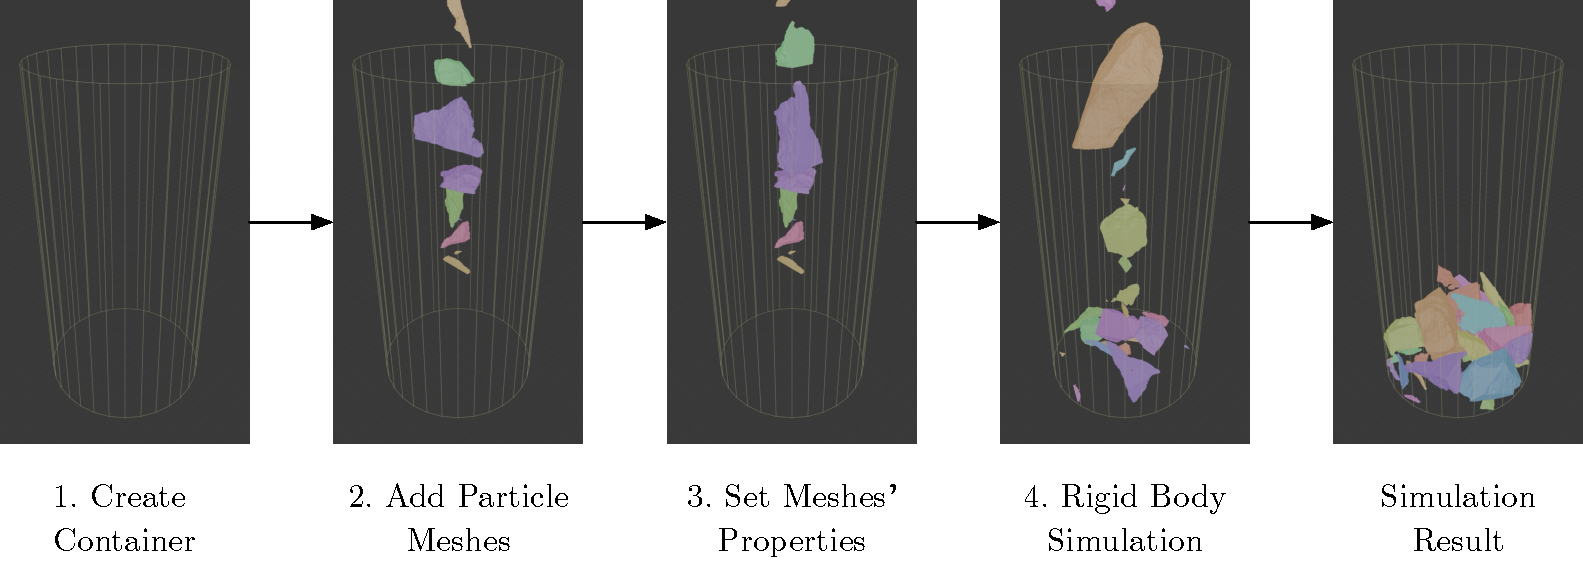
\includegraphics[width=\textwidth]{figures/pdf/simulation-pipeline.pdf}
    \caption{Pipeline of Batched Rigid Body Simulation}
    \label{fig:batched_rigid_body_simulation_pipeline}
\end{figure}
\par
The batched rigid body simulation pipeline, depicted in \cref{fig:batched_rigid_body_simulation_pipeline}, begins by creating a tube—a container resembling the one used in CT scans. 
We then introduce a set of particle meshes into the simulation environment and assign their properties, including weight, gravitational centre, initial position, and scale (the detail will be shown in \ref{subsubsec:syn:simu:imp_detail}). 
Following this, the rigid body simulation is initiated. 
After a specified number of time steps, once the particle meshes have settled, the position and orientation of particles are fixed to prevent particles from performing minor adjustments or ``damping'', which could significantly affect the performance.
This step guarantees that the simulation stays both manageable and scalable, especially crucial when dealing with large quantities of particles, as minor adjustments would otherwise lead to a significant increase in unnecessary computational work.
Importantly, it does not significantly compromise the effectiveness of the simulations.
Lastly, another simulation batch can be initiated for larger generated tomogram or the simulation process concludes and outputs the simulation result. 
The final simulation result will contain the translation and the rotation of each particle mesh.
\subsubsection{Choice of Simulation}
Rigid body simulation is chosen for simulating particle pack processes because it efficiently handles the complexity of shapes and inter-particle dynamics essential for accurately representing hard, non-deformable particles. 
Unlike soft body simulations, which are better suited for scenarios involving material deformation or bending, rigid body simulation is optimal for processes where particles maintain their shape, as it avoids the unnecessary computational costs associated with modelling deformations. 
Additionally, while particle simulations might simplify particles to point masses \footnote{A point mass is an object of negligible size, treated as if all its mass is concentrated at a single point in space for the purposes of modelling.} by ignoring the geometry of particle to make the simulation more efficient and scalable, rigid body simulation takes into account the geometric details of each particle. 
This enables a more precise representation of packing, collisions, and stacking behaviours critical to the process, making rigid body simulation a more efficient and realistic method for simulating particle pack processes.
\subsubsection{Choice of Simulator}
Blender was selected to perform batched rigid body simulation, driven by the need for a tool that offered a graphical user interface (GUI) for visualisation, a scripting interface for automation, and was relatively efficient.
% \begin{table}[h!]
%     \centering
%     \begin{tabularx}{\textwidth}{|c|c|c|c|>{\centering\arraybackslash}X|}
%         \hline
%         \textbf{Simulation Tool} & \textbf{GUI} & \textbf{Efficiency} & \textbf{Scripting Interface} & \textbf{Open Sourced} \\ \hline
%         Blender                  & \cmark       & High                & \tt{Python}                  & \cmark                \\ \hline
%         Bullet Physics           & \xmark       & High                & \tt{Python}, \tt{C++}        & \cmark                \\ \hline
%         Unity 3D                 & \cmark       & Medium              & \tt{C\#}                     & \xmark                \\ \hline
%         Unreal Engine            & \cmark       & Medium              & \tt{C++}                     & \xmark                \\ \hline
%         PhysX by NVIDIA          & \xmark       & Very High           & \tt{C++}                     & \xmark                \\ \hline
%     \end{tabularx}
%     \\
%     \begin{tabular}{|c|l|}
%         \hline
%         \textbf{Simulation Tool} & \multicolumn{1}{c|}{\textbf{Additional Features}}                                                                                                                   \\ \hline
%         Blender                  & \begin{tabular}[c]{@{}l@{}}Well-suited for 3D modelling, animation, and simulation; \\ Large community support; integrates well with other tools.\end{tabular}      \\ \hline
%         Bullet Physics           & \begin{tabular}[c]{@{}l@{}}Real-time physics simulation, including rigid body dynamics; \\ Widely used in both academic research and game development.\end{tabular} \\ \hline
%         Unity 3D                 & \begin{tabular}[c]{@{}l@{}}Game engine with comprehensive tools for simulation, \\ visualisation, and game development.\end{tabular}                                \\ \hline
%         Unreal Engine            & \begin{tabular}[c]{@{}l@{}}Similar to Unity 3D, but a different scripting interface. \end{tabular}                                                                  \\ \hline
%         PhysX by NVIDIA          & \begin{tabular}[c]{@{}l@{}}High-performance physics engine. \end{tabular}                                                                                           \\ \hline
%         \end{tabular}%
%     \caption{Comparison of Tools for Rigid Body Simulation}
%     \label{tab:syn:comparison_tool_rigid_body_simulation}
% \end{table}
\par
% It stood out among alternatives like Bullet Physics, Unity 3D, Unreal Engine, and PhysX by NVIDIA, according to our evaluation presented in the \cref{tab:syn:comparison_tool_rigid_body_simulation}.
Compared to PyBullet, Blender's GUI enables visualisation of simulations, facilitating a more intuitive interaction with the simulation environment.
In our study, Python served as the primary programming environment for the broader project, using Python ensuring a consistent and unified programming interface.
Unity 3D and Unreal Engine, with their comprehensive suites of development tools and GUIs, are ideal for projects that require advanced visualisation and interactive simulation capabilities, though with some trade-offs in scripting flexibility and open-source accessibility. 
PhysX, known for its high-performance via GPU acceleration in various simulations, is best suited for projects that require high efficiency, but its platform dependency can potentially hinder cross-platform compatibility. 
\subsubsection{Implementation Detail} \label{subsubsec:syn:simu:imp_detail}
In simulation of the particle packing processes, specific settings and procedures are crucial to achieving accurate and reproducible results. 
This part provides a detailed overview of the implementation specifics used in our simulations, focusing on the settings of the gravitational center, particle properties, and the locking mechanism of the particles.
\begin{itemize}
    \item 
    The gravitational center plays a pivotal role in our simulation. 
    It is established at the center of the mesh, determined by calculating the object's surface area \citep{blender2023objectops}. 
    This configuration ensures that gravitational effects are realistically simulated, mirroring the natural behavior of particles under the influence of gravity. 
    For ease of reconstruction after exporting the simulation results, the center of the object is repositioned to align with the center of the original bounding box.
    \item
    In our implementation, the mass of each particle is estimated based on particles density and the size of the mask, as illustrated in \cref{eqn:mass}
    \begin{align}
        \text{mass} &= \rho V \label{eqn:mass}
    \end{align}
    where $\rho$ is the density of a particle, $V$ is the volume of a particle mask.
    This method provides a rapid approximation of weight, suitable for scenarios where detailed precision is less critical. 
    \item
    The initial positioning and scaling of particles are highly dependent on the experimental setup. 
    Adjustments to the initial position can significantly affect the final placement of particles within the volume. 
    Similarly, changing the scale influences the packing density (how tightly particles are packed together), resembling different particle packing configurations.
    \item 
    As noted above, simulation in batches will enhance the overall performance and manageability. 
    A unique feature of our workflow is the locking mechanism employed after each batch.
    The particle locking is realised by key frame feature in Blender.
    Key frames are used extensively in animation and simulation to mark specific points at which certain properties of an object are saved. 
    In our context, we introduce a key frame between two consecutive time steps, $t$ and $t + 1$, 
    At time $t$, particles from the previous batch are still moveable, allowing them to perform rigid body simulation.
    At time $t+1$, a new batch of particles is introduced into the simulation environment;
    Simultaneously, movement of particles from the previous batch is disabled. 
    This ``locking'' of particles after each batch prevents any further adjustments, ensuring stability and reducing computational overhead, particularly when handling a large number of particles.
\end{itemize}
%===============================================================================
\subsection{Simulation Reconstruction}
Given the results of the simulation, the particle pack can be constructed within the tomogram by repositioning each particle. 
% As shown in \cref{alg:syn:reconstruct}, 
The construction process involves initially gathering volumetric data from the particles' tomograms and masks, alongside the simulation outcomes from batched rigid body simulations. 
Subsequently, arrays that represents the reconstructed tomogram and its mask are generated. 
The reconstruction then proceeds in parallel, commencing with the creation of each particle's rotation and translation matrix, followed by the acquisition of volumetric data for the tomogram and mask of each particle. 
Finally, each particle is rotated and positioned within the resulting tomogram and mask.
% \begin{algorithm}
%     \SetKwFor{ParallelFor}{parallel for}{do}{end parallel for}
%     \caption{Reconstruct(\it{ParticleTomograms}, \it{ParticleMasks}, \it{ParticlePlacements})}\label{alg:syn:reconstruct}
%     \DontPrintSemicolon
%     \KwIn{A list of particle tomograms with their masks (\it{ParticleTomograms}, \it{ParticleMasks}), and their placements (\it{ParticlePlacements})}
%     \KwOut{Reconstructed tomogram with its mask}
%     Let \it{n} be the number of particles involved in the simulation \;
%     Let \it{resultTomogram} be the reconstructed tomogram \;
%     Let \it{resultMask} be the reconstructed mask \;
%     \ParallelFor {$1 \le \it{particleIndex} \le n$} {
%         \it{particleRotation} = \it{ParticlePlacements}[\it{particleIndex}].\it{rotation} \;
%         \it{particleTranslation} = \it{ParticlePlacements}[\it{particleIndex}].\it{translation} \;
%         \it{particleTomogram} = \it{ParticleTomograms}[\it{particleIndex}] \;
%         \it{rotatedTomogram} = \tt{Rotate}(\it{particleTomogram}, \it{particleRotation}) \;
%         \tt{Place}(\it{rotatedTomogram}, \it{particleTranslation}, \it{resultTomogram}) \;
%         \it{particleMask} = \it{ParticleMask}[\it{particleIndex}] \;
%         \it{rotatedMask} = \tt{Rotate}(\it{particleMask}, \it{particleRotation}) \;
%         \tt{Place}(\it{rotatedMask}, \it{particleTranslation}, \it{resultMask}) \;
%     }
% \end{algorithm}

Building on the process of reconstructing the particle pack within the tomogram, we next focus on the methodology for rotating tomograms and masks. 
To achieve rotation, a rotation matrix is constructed based on the specified rotation angles along the $x$, $y$, and $z$ axes, employing separate rotation matrices for each axis. 
The matrix for rotation about the $x$, $y$ and $z$-axis is defined as \eqref{eqn:syn:rx}, \eqref{eqn:syn:ry} and \eqref{eqn:syn:rz} respectively:
\begin{align}
    R_x(\theta) &= \begin{bmatrix} 1 & 0 & 0 \\ 0 & \cos(\theta) & -\sin(\theta) \\ 0 & \sin(\theta) & \cos(\theta) \end{bmatrix}; \label{eqn:syn:rx} \\
    R_y(\phi)   &= \begin{bmatrix} \cos(\phi) & 0 & \sin(\phi) \\ 0 & 1 & 0 \\ -\sin(\phi) & 0 & \cos(\phi) \end{bmatrix}; \label{eqn:syn:ry} \\
    R_z(\psi)   &= \begin{bmatrix} \cos(\psi) & -\sin(\psi) & 0 \\ \sin(\psi) & \cos(\psi) & 0 \\ 0 & 0 & 1 \end{bmatrix}. \label{eqn:syn:rz}
\end{align}
The comprehensive rotation matrix, integrating rotations about all three axes, is derived by multiplying the individual matrices in the sequence \(R = R_z(\psi)R_y(\phi)R_x(\theta)\). 
To retain the original 3D volume after rotation and ensure that no part of the image is lost, padding is necessary. 
The process can be understood in three main steps:
\begin{enumerate}
    \item Each vertex \( V_i \) of the bounding box of the volume is transformed using the combined rotation matrix \( R \) to obtain its new position \( V_i' \):
    \begin{align}
        V_i' = R \cdot V_i,
    \end{align}
    where \( V_i \) is a vector representing the coordinates of the \textit{i}-th vertex of the volume's bounding box. 
    \item After the rotation, the dimensions of the bounding box are determined by calculating the minimum and maximum values of the transformed vertices' coordinates along each axis. 
    The differences between these values give us the dimensions of the bounding box:
    \begin{align}
    L &= \lceil \max(X') - \min(X') \rceil; \\
    W &= \lceil \max(Y') - \min(Y') \rceil; \\
    H &= \lceil \max(Z') - \min(Z') \rceil, 
    \end{align}
    where $X'$, $Y'$ and $Z'$ are the x, y, and z-coordinates of rotated vertices.
    \item Finally, the size of padding applied to each direction can be calculated as:
    \begin{align}
        \text{$x$ direction padding} &= 2 \times (L - L_0); \\
        \text{$y$ direction padding} &= 2 \times (W - W_0); \\
        \text{$z$ direction padding} &= 2 \times (H - H_0),
    \end{align}
    where $L_0$, $W_0$ and $H_0$ are the original size of the volume's bounding box.
\end{enumerate}
This padding step ensures that the original volume is completely enclosed within the new dimensions post-rotation, preserves the integrity of the 3D volume.
Lastly, having this rotation matrix and the size after rotation, an affine transformation with interpolation is then applied to the original tomogram and mask to generate a rotated particle volume. 

%===============================================================================
\subsection{Post-processing}
Post-processing plays a crucial role in bridging the gap between synthetic and real-world data, enhancing the realism of synthetic tomograms. 
As real tomograms are rarely perfect, they often contain defects resulting from equipment limitations, photon scarcity, or environmental interference. 
\par
One fundamental post-processing step is the addition of noise. 
Gaussian noise, speckle noise, and Poisson noise are commonly added to replicate these real-world imperfections, thereby produce a more realistic synthetic data.
Another aspect of realism is the presence of artefacts, which can also be deliberately introduced into synthetic tomograms. 
These artefacts might include motion blur, ring effects, or beam hardening, which are common in tomographic imaging. 
By simulating these artefacts, synthetic datasets can closely mimic the challenges faced when processing real-world data, providing an invaluable ground truth for developing algorithms robust to these artefacts.
An example of the post-processed synthesised slice is shown in \cref{fig:syn:postprocess}. 
After post-processing, the synthetic slice appears more realistic.
\begin{figure}[H]
    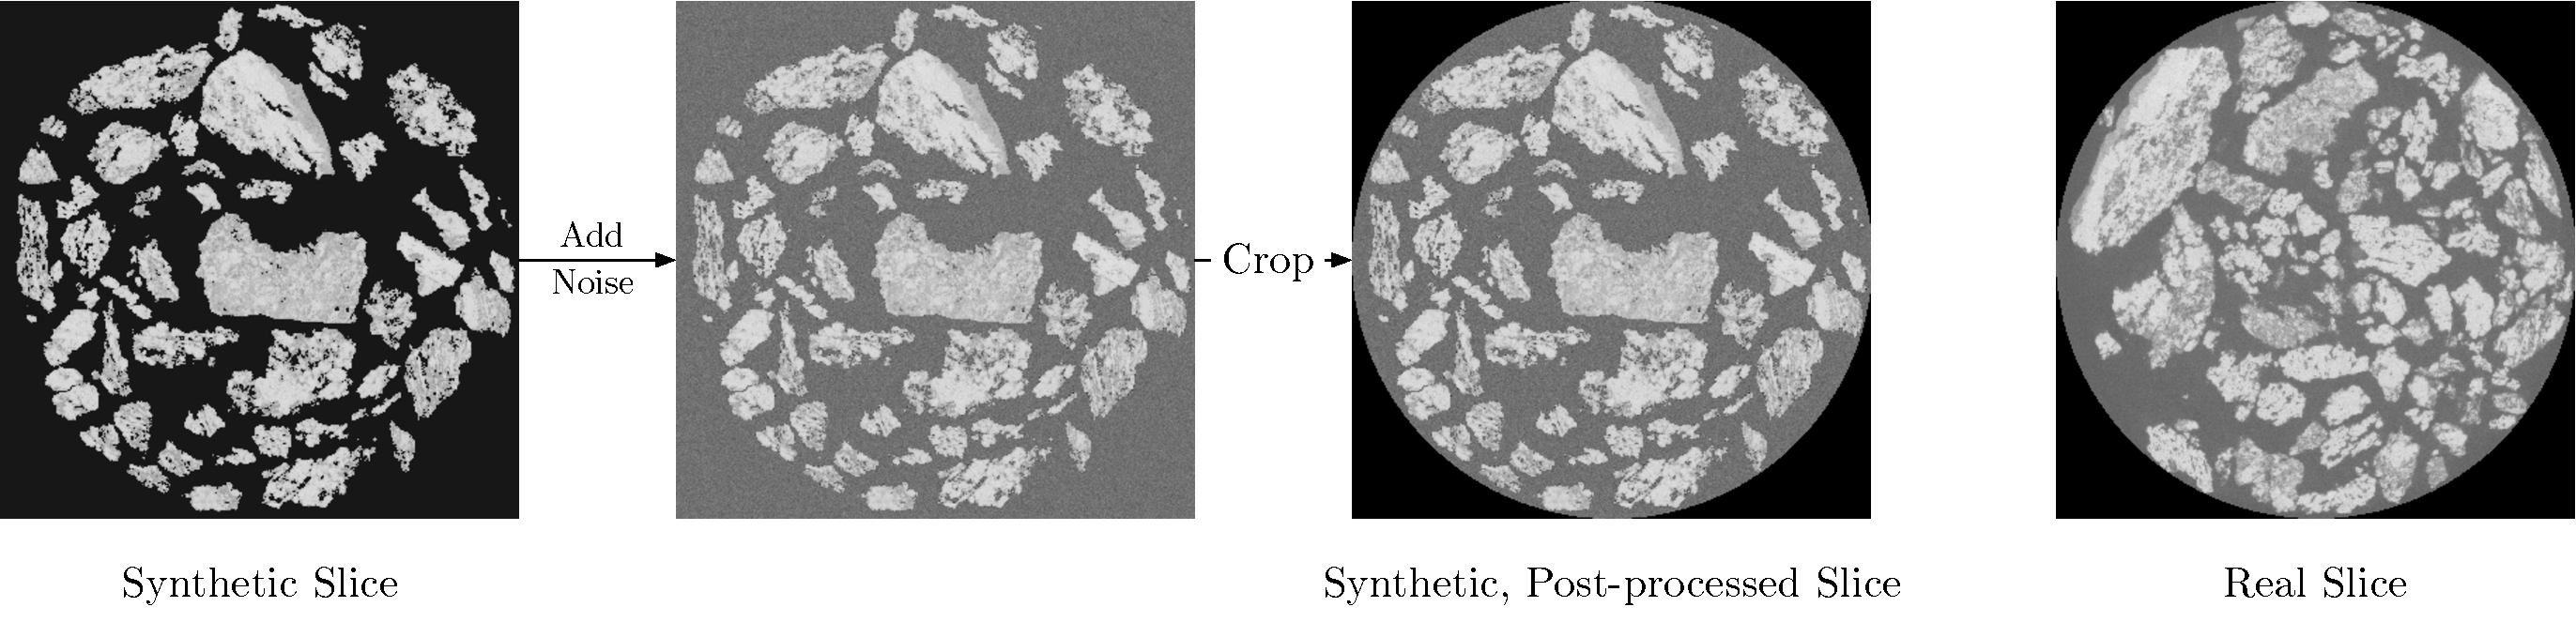
\includegraphics[width=\textwidth]{figures/pdf/postprocess.pdf}
    \caption{An Example of Postprocessing Slice in Simulated Particle Pack Data}
    \label{fig:syn:postprocess}
\end{figure}

\section{Experiment \& Discussions}

Having constructed synthetic particle packs as described in \Cref{sec:method}. 
We will conduct a couple of experiments to investigate the efficacy of using synthetic particle packs to augment existing training datasets for 2D particle segmentation.
This augmentation approach is particularly valuable for scenarios where acquiring large volumes of real data is impractical due to constraints such as cost, time, or accessibility. 
As synthetic data can be designed to cover a wide range of variations and complexities not always present in real-world data, potentially filling gaps in the dataset that hinder the model's ability to learn diverse features and scenarios.

\subsection{Experiment Setup}
% YOLOv8-seg is selected for 2D segmentation in this experiment due to its simplicity in deployment.
% To effectively evaluate our method, we partitioned the real datasets into training and testing subsets. 
To effectively train and evaluate our model, we partitioned each tomogram into training and testing sets. 
We specifically avoided random selection of slices for the testing set due to the high similarity between consecutive slices within the particle pack. 
This similarity can lead to overestimation of model performance, as the model might simply be recognising similar instances it has already encountered in adjacent slices, rather than generalising from diverse examples. 
Therefore, we allocated the central 20\% of the particle pack slices to the testing set, and the remaining 80\% for training.
This will avoid the similarity between training set and testing set. 

In this experiment, the YOLOv8m-seg model from Ultralytics \citep{jocher2023yolo} will be employed due to its versatility across a wide range of applications as well as optimal balance between computational speed and segmentation accuracy.

Lastly, we selected the Dice score \cite{Dice1945MeasuresOT}, also known as Dice-Sørensen coefficient (shown in \cref{eqn:dice}) to evaluate segmentation performance of trained models.
As it effectively evaluating segmentation accuracy by accounting for both false positives and false negatives, providing a balanced view of under and over-segmentation.
\begin{align}
    \label{eqn:dice}
    \text{Dice Score} = 2 \times \frac{\text{Area of Overlap}}{\text{Total Area}}
\end{align}

\subsection{Result I: Synthetic Data Improves Segmentation Accuracy}
To assess performance improvements with synthetic particle packs, we trained and tested segmentation models using real data alone, and real data augmented with synthetic particle pack data. 
The results for each model, presented in \Cref{tab:res1}, demonstrate that incorporating synthetic data consistently improves segmentation performance for both large and small particles.
Specifically, when trained with real large particles augmented with synthetic data, the accuracy increased from 94.5\% to 96.0\% for large particles and from 92.4\% to 94.8\% for small particles. 
Similarly, training with real small particles combined with synthetic data improved the accuracy on large particles from 77.0\% to 80.1\%, while the improvement for small particles was more modest, rising from 90.1\% to 90.9\%. 
These results indicate that synthetic data enriches the training set with diverse examples, thereby enhances the model's ability to segment tomograms with different particle sizes. 
% the model's performance increased with the addition of synthetic datasets. 
% Specifically, from the first entry of \cref{tab:res1}, datasets contains large particles augment with synthetic data resulted in a more significant performance improvement on small particles.
% Similarly, from the second entry of \cref{tab:res1}, large particles gained a more pronounced improvement compared to the small particles. 
% This can be explained as the incorporation of synthetic data enriched the real datasets with unseen examples. 
% This enrichment allowed the model to learn more diverse features, improving its generalisation ability.
\begin{table}[]
    \center
    \begin{tabular}{|l|l|l|}
        \hline
                                 & Real Large & Real Small \\ \hline
        Real Large               & 94.5\%     & 77.0\%     \\ \hline
        Real Large + Syn         & 96.0\%     & 80.1\%     \\ \hline
        Real Small               & 92.4\%     & 90.1\%     \\ \hline
        Real Small + Syn         & 94.8\%     & 90.9\%     \\ \hline
    \end{tabular}
    \caption{Testing results for different tomogram datasets. 
    Each row represents the training set and each column represents the testing set. 
    Real Large refers to a real tomogram dataset with large particles, while Real Small refers to a real tomogram dataset with small particles. 
    Rows include results from training on only the real datasets and combinations with synthetic data (Real Large + Syn, Real Small + Syn). 
    Columns indicate testing on real datasets with large or small particles.}
    \label{tab:res1}
\end{table}

\subsection{Result II: Postprocessing Is Crucial In Augmentation}
In our experiment, the postprocessing involved adding gaussian noise to the synthetic data. 
The observed results from \Cref{tab:res2} indicate that after adding noise, the training dataset was successfully augmented, leading to improvements in the models' performance across various test sets. 
Conversely, without adding noise, the models' performance sometimes degraded, as evidenced by decreases in Dice scores in certain cases.

This can be attributed to the noise making the synthetic slices more realistic and closer to the actual data the model will encounter, thereby reducing the domain gap between synthetic and real data.
Without noise, the synthetic data lacks the necessary realism, leading the model to learn features that do not transfer well to real-world scenarios.
This discrepancy can cause the model to perform poorly on real data, effectively learning in a different domain than the one it is tested on. This highlights the importance of appropriate postprocessing to make synthetic datasets more realistic, which enhances its utility for augmenting existing datasets.

\begin{table}[]
    \center
    \begin{tabular}{|l|l|l|l|l|}
    \hline
                                        & Real Large & Real Small \\ \hline% & Real Large Particles + Small Particles & Real Small Particles + Synthetic Large Particles \\ \hline
    Real Large + Syn w/ Postprocessing  & 96.0\%     & 80.1\%               \\ \hline% &                                        &                                                  \\ \hline
    Real Large + Syn w/o Postprocessing & 94.9\%     & 76.9\%               \\ \hline% &                                        &                                                  \\ \hline
    Real Small + Syn w/  Postprocessing & 94.8\%     & 90.9\%               \\ \hline% &                                        &                                                  \\ \hline
    Real Small + Syn w/o Postprocessing & 92.4\%     & 88.8\%               \\ \hline% &                                        &                                                  \\ \hline
    \end{tabular}
    \caption{Testing results for real tomogram datasets with large and small particles using different training sets, with and without postprocessing. Each row indicates a different training configuration: Real Large + Syn or Real Small + Syn, combined with postprocessing (w/) or without postprocessing (w/o). Columns show testing results on real datasets: Real Large and Real Small. Performance varies depending on the use of postprocessing and particle size of the testing set.}
    \label{tab:res2}
\end{table}



\section{Conclusion}
This paper presents a comprehensive workflow for generating synthetic particle pack datasets through physics-based simulation. 
Our approach addresses the challenges of acquiring accurate CT tomograms and segmentation ground truths for training and evaluation of segmentation algorithms by leveraging simulations to produce enriched and realistic datasets. 
% By modelling the physical packing process, we enhance the precision and efficiency of particle segmentation in various scientific fields. 
The integration of noise and artefacts in post-processing further bridges the gap between synthetic and real-world data, offering a data generation platform for future research. 
\par
Our experimental results validate the effectiveness of our synthetic particle pack generation workflow. 
By augmenting real datasets with synthetic data, we achieved consistent improvements in segmentation accuracy across different particle sizes, as demonstrated by higher Dice scores in \Cref{tab:res1}. 
The integration of post-processing techniques, specifically the addition of noise, was crucial in bridging the gap between synthetic and real-world data, leading to enhanced model performance (\Cref{tab:res2}). 
These findings highlight the potential of our approach to enrich annotated particle pack data for training and validation of segmentation algorithms.
\par
In the current synthetic particle-pack-generation workflow, we rely on manually labelled particle packs, which limits the versatility of the particle data. 
To eliminate this dependency and increase data diversity, we propose two improvement directions. 
The first approach involves using classical methods such as free-form deformation (FFD) \cite{sederberg1986free} to alter particles' shape while retaining their core characteristics. 
This method is relatively fast, easy, and deterministic but still relies on the existing particle data.
The second approach involves employing advanced machine-learning techniques, such as diffusion models \cite{ho2020denoising} or generative adversarial networks (GANs) \cite{goodfellow2014generativea}. 
These models would first learn the features of the particle data and then generate entirely synthetic particle data. 

%% The Appendices part is started with the command \appendix;
%% appendix sections are then done as normal sections
% \appendix

% \section{Sample Appendix Section}
% \label{sec:sample:appendix}
% Lorem ipsum dolor sit amet, consectetur adipiscing elit, sed do eiusmod tempor section \ref{sec:introduction} incididunt ut labore et dolore magna aliqua. Ut enim ad minim veniam, quis nostrud exercitation ullamco laboris nisi ut aliquip ex ea commodo consequat. Duis aute irure dolor in reprehenderit in voluptate velit esse cillum dolore eu fugiat nulla pariatur. Excepteur sint occaecat cupidatat non proident, sunt in culpa qui officia deserunt mollit anim id est laborum.

%% If you have bibdatabase file and want bibtex to generate the
%% bibitems, please use
%%
 \bibliographystyle{elsarticle-num} 
 \bibliography{cas-refs}

%% else use the following coding to input the bibitems directly in the
%% TeX file.

% \begin{thebibliography}{00}

% %% \bibitem{label}
% %% Text of bibliographic item

% \bibitem{}

% \end{thebibliography}
\end{document}
\endinput
%%
%% End of file `elsarticle-template-num.tex'.
